\documentclass[presentation]{beamer}

\usepackage{graphicx}
\usepackage{multirow}
\usepackage{amsmath,amssymb,amsfonts}
\usepackage{amsthm}
\usepackage{mathrsfs}
\usepackage[title]{appendix}
\usepackage{xcolor}
\usepackage{textcomp}
\usepackage{manyfoot}
\usepackage{booktabs}
\usepackage{algorithm}
\usepackage{algorithmicx}
\usepackage{algpseudocode}
\usepackage{listings}
\usepackage{float}
\usepackage{hyperref}


\usepackage[utf8]{inputenc}
\usepackage[T1]{fontenc}
\usepackage{graphicx}
\usepackage{longtable}
\usepackage{wrapfig}
\usepackage{rotating}
\usepackage[normalem]{ulem}
\usepackage{amsmath}
\usepackage{amssymb}
\usepackage{capt-of}
\usepackage{hyperref}
\newcommand{\mycomment}[1]{}

\usetheme{default}
\author{Sergi Simón Balcells}
\date{2025/04/01}
\title{A quantum-resistant unlinkable and strongly-unsplittable multi-coupon system}
\subtitle{\#ProyectosCiber}
\makeatletter
\newlength\beamerleftmargin
\setlength\beamerleftmargin{\Gm@lmargin}
\makeatother
\begin{document}

\begin{frame}
  \titlepage
  \begin{figure}
    \hspace*{-\beamerleftmargin}%
    
\includegraphics[width=\paperwidth]{incibe.jpg}
  \end{figure}
\end{frame}

\begin{frame}
  \frametitle{Acknowledgements}
  Esta investigación resulta del Proyecto Estratégico 'Avances
  en criptografía post-cuántica aplicados al desarrollo
  de un sistema de cupones' (C039/24), fruto del convenio
  de colaboración suscrito entre el Instituto Nacional de
  Ciberseguridad (INCIBE) y la Universidad de Lleida. Esta
  iniciativa se realiza en el marco de los fondos del Plan de
  Recuperación, Transformación y Resiliencia, financiados
  por la Unión Europea (Next Generation).
\end{frame}


  \begin{frame}{Outline}
    \tableofcontents
  \end{frame}

\section{Multi-coupon system}
% TODO: diagrama de com un cupó porta al seguent i 
%   amb mes descompte
% - Explicar que son s'encripta les claus i amb una operació
%   que nomes l'issuer pot fer es deslliga al seguent.

\begin{frame}
  \frametitle{Multi-coupon system}
\begin{figure}
  \begin{center}
    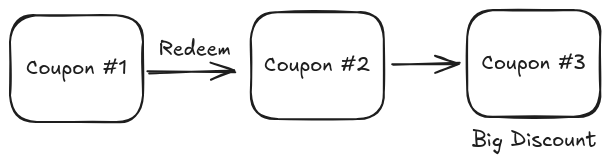
\includegraphics[width=0.95\textwidth]{multi-coupon}
  \end{center}
  \caption{Schematic of a multi-coupon system}\label{fig:multi-coupon}
\end{figure}
\end{frame}

\begin{frame}
  \frametitle{Multi-coupon redeem}
\begin{figure}
  \begin{center}
    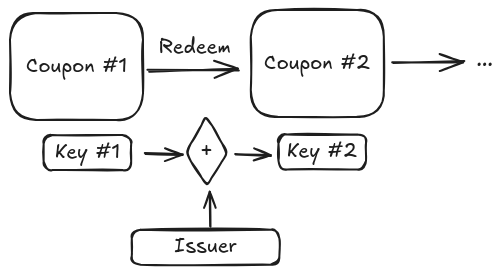
\includegraphics[width=0.95\textwidth]{redeem-token}
  \end{center}
  \caption{Redeem token with the issuer.}\label{fig:redeem-token}
\end{figure}
\end{frame}

\section{Privacy Questions}
% TODO: cita in-proceedings ?
\begin{frame}{Privacy Requirements}
 \begin{enumerate}
   \item The multi-coupon system is \alert{strongly unsplittable}.
     \pause
   \item The tokens redeemed are \alert{unlinkable}.
     \pause
   \item The tokens are \alert{unforgeable}.
     \pause
   \item The employed cryptography is \alert{quantum-resistant}.
 \end{enumerate}
\end{frame}

\section{A Post-Quantum Approach: Results}
\begin{frame}
  \frametitle{A Post-Quantum Approach: Results}
  \begin{table}[!h]
    \caption{Running times in milliseconds (ms) of the procedures composing the multi-coupon system.}\label{tab:results}
    \centering
    \begin{tabular}[c]{r|lll}
      \toprule
      Processor & Set up & Token creation & Token redemption \\
      \midrule
      i7-6700HQ    & 13059.45 & 127.07 & 150.46 \\
      Ryzen 5 3600 & 9258.17 & 103.41 & 125.29 \\
      i7-9700K     & 9249.97 & 93.80 & 111.69 \\
      i7-12700H    & 4949.05 & 60.89 & 79.41 \\
      \botrule
    \end{tabular}
  \end{table}
  \begin{itemize}
    \item Python and SageMath implementation.
    \item Network cost is 0.
  \end{itemize}
\end{frame}


\section{Future Work}
% TODO: ??? Que falta per fer?
% - I don't know




\begin{frame}
  \huge{Thanks for your attention}
\end{frame}

% NOTE: I have no refereces
% \begin{frame}[allowframebreaks]
%   \frametitle{References}
%   \bibliographystyle{apalike}
%   \bibliography{bib}
% \end{frame}

\end{document}

